\documentclass[11pt,a4paper]{article}
\usepackage[margin=25mm]{geometry}
\usepackage[T1]{fontenc}
\usepackage{lmodern,microtype}
\usepackage{amsmath,amssymb,booktabs,graphicx,array,longtable}
\usepackage{xcolor,xurl,caption,fancyhdr,needspace}
\usepackage[section]{placeins}
\usepackage{hyperref}
\definecolor{paperlink}{RGB}{24,60,91}
\hypersetup{colorlinks=true,urlcolor=paperlink,citecolor=paperlink,linkcolor=paperlink,
 pdftitle={Separating Training Exposure from Data Scarcity in MuSGD-YOLO Fine-Tuning under Missing Annotations},
 pdfauthor={Muchammad Yuda Tri Ananda},
 pdfsubject={Empirical object detection optimizer comparison with fixed image exposure},
 pdfkeywords={object detection, MuSGD, YOLO26, missing annotations, data scarcity}}
\captionsetup{font=small,labelfont=bf}
\setlength{\emergencystretch}{2em}
\setlength{\parskip}{0.2em}
\setlength{\textfloatsep}{14pt plus 3pt minus 3pt}
\renewcommand{\arraystretch}{1.12}
\widowpenalty=10000
\clubpenalty=10000
\pagestyle{fancy}
\fancyhf{}
\fancyhead[L]{\small MuSGD--YOLO fine-tuning}
\fancyhead[R]{\small M.\,Y.\,T.\ Ananda}
\fancyfoot[C]{\thepage}
\renewcommand{\headrulewidth}{0.3pt}
\setlength{\headheight}{14pt}
\title{Separating Training Exposure from Data Scarcity in MuSGD--YOLO Fine-Tuning under Missing Annotations}
\author{Muchammad Yuda Tri Ananda\\[3pt]\normalsize\href{mailto:yuda@myudak.com}{\texttt{yuda@myudak.com}}}
\date{31 October 2026}
\begin{document}
\maketitle
\thispagestyle{plain}
\begin{abstract}
Limited training images and missing bounding boxes jointly constrain detector fine-tuning, while fixed ordinary epochs also change update count across dataset fractions. We compare existing MuSGD, AdamW and momentum-SGD recipes in pretrained YOLO26n using fixed image exposure, validation-only candidate selection and paired training/subset/deletion randomizations. Each primary run receives 20,480 image presentations and 1,280 updates, crossing 20\%/100\% image availability with 0\%/20\% independent box deletion. Three joint blocks cover African Wildlife and a VOC2007-derived all-object transfer task; VOC settings are transferred without retuning. The campaign completed 120 training trials and 60 frozen-checkpoint test evaluations. MuSGD--AdamW test differences range from $-0.25$ to $+0.79$ AP points on wildlife and $+0.73$ to $+1.67$ on VOC-derived data. The scarcity--missingness interaction is $+0.47$ points on wildlife (approximate paired 95\% interval $[-6.38,7.32]$) and $+0.49$ on VOC-derived data ($[-0.66,1.64]$), leaving the joint interaction unresolved. All selected learning rates lie at the lower search boundary, and the prespecified extension was skipped by the runtime-reservation rule. These results document dataset-dependent recipe behavior under a short adaptation budget; wider search coverage and stronger replication are needed for broader conclusions.
\end{abstract}
\noindent\textbf{Keywords:} object detection; MuSGD; YOLO26; missing annotations; data scarcity; fixed exposure.


\section{Introduction}
Detector training with missing bounding boxes can treat visible but unannotated objects as background. This is an established positive--unlabeled learning problem \cite{yang2020}. Independently, a smaller image pool restricts the variety of scenes and objects available for adaptation. Fixed-epoch experiments couple these data changes to update count: a smaller pool produces fewer optimizer steps.

Muon and its mixed variants already have precedents in vision and object detection \cite{jordan2024,jocher2026,huang2026}. This study therefore evaluates existing fine-tuning recipes rather than introducing an optimizer. We quantify how recipe differences vary with available images and missing training annotations while holding presented-image exposure and update count constant. Budget matching itself is also established methodology \cite{akhtar2026}.

The primary question is descriptive: at a fixed short adaptation budget, does the MuSGD--AdamW difference depend jointly on image scarcity and missing-box probability? Momentum SGD is a secondary baseline. The protocol was developed after the pilot, and no directional hypothesis was preregistered. The later randomized blocks provide separate evidence for the fixed-exposure comparison.

\section{Related work}
Muon applies orthogonalized matrix updates \cite{jordan2024}. Ultralytics YOLO26 combines Muon and SGD updates in its MuSGD training recipe \cite{jocher2026}; MiMuon is another mixed optimizer with detector experiments \cite{huang2026}. Matrix-based updates in object detection are therefore established. Our comparison concerns the existing library recipes during fine-tuning, with controlled image availability and training-box deletion.

Budget definitions affect optimizer comparisons. Akhtar et al.\ distinguish matched-data, elapsed-time and tuning-budget evaluations \cite{akhtar2026}. Here, primary cells receive equal image presentations and updates, while timings include the surrounding training and validation pipeline. Equal candidate counts constrain the search budget but do not ensure equally complete search coverage.

Ruan et al.\ study input-corruption robustness and feature transfer \cite{ruan2026}. The present intervention instead removes training annotations while retaining the original images. Fine-tuning also depends on checkpoint lineage: Qu et al.\ investigate switching from Adam pretraining to Muon \cite{qu2026}. Our fixed YOLO26 checkpoint records MuSGD pretraining, so an Adam-pretraining mismatch explanation does not directly apply.

Missing-box learning is an established positive--unlabeled detection problem \cite{yang2020}. Annotation-incompleteness studies further distinguish controlled synthetic deletion from natural omissions and ambiguous labels \cite{penquitt2026}. We evaluate unchanged retained source annotations, with independent deletion applied only to training labels. The resulting VOC-derived metric is explicitly separate from standard VOC evaluation \cite{everingham2010}.

\section{Methods}
\subsection{Study phases and provenance}
The development pilot and journal campaign are separate phases. The pilot used one joint realization and provisional learning rates. The later protocol, source bundle, checkpoint hashes and split identities are saved before journal training. Superseded development jobs are retained in a run registry and excluded from pooled estimates. All GPU training is executed on Kaggle; the local computer is used for source editing and CPU checks.

\subsection{Data and split handling}
The African Wildlife download \cite{wildlifeData} contains 1,052/225/227 training/validation/test images. An exact-content audit and a hash-bound review of 12 additional training near copies produced the pilot pool of 1,021/223/227 images, with 1,881/377/375 annotated objects. Test membership was unchanged. Retained annotations were unchanged; the scene audit was not exhaustive.

The journal phase additionally prespecifies a conservative cross-split image screen: dHash distance at most 6, RGB mean absolute error at most 0.025 after resizing to $32\times32$, and relative aspect change at most 0.05. Connected components retain the highest-priority split, ordered test, validation, then training. Same-split duplicates may remain. A subsequent input-only review of preflight candidate sheets identified one likely same-scene wildlife training image outside the automatic RGB threshold. Its conservative exclusion was bound to source and peer hashes before main submission, without using preflight scores. The frozen journal pool contains 1,020/223/227 images and 1,880/377/375 objects; the pilot remains unchanged.

The external task uses the official VOC2007 train, validation and test membership \cite{everingham2010} before the same screen (2,501/2,510/4,952 images). All annotated objects, including difficult objects, are retained. One-based inclusive boxes are converted to zero-based half-open bounds and normalized. Evaluation uses all-object mAP50--95, not official VOC AP. A deterministic validation sample of 512 images is fixed without model outcomes and contains all 20 classes. The frozen train/validation/test counts are 2,501/512/4,952 images and 7,844/1,591/14,976 objects. Full original test membership is retained. Dataset terms remain those of the original providers; possible overlap with pretraining data is not excluded.

\subsection{Scarcity and annotation deletion}
For fraction $f\in\{0.2,1.0\}$, a SHA-256 ranking of source-relative paths and a subset seed selects the first $\lceil fN\rceil$ training images. Fractions are nested within a joint block and are not class stratified. For each original object, a deterministic score derived from image path, object index and deletion seed removes its box with target probability $q\in\{0,0.2\}$. The realized deletion rate is removed boxes divided by original boxes in the selected subset. Images with no remaining boxes are retained. Validation and test annotations are not corrupted. All optimizer recipes share the exact same variant within each paired block and condition.

\subsection{Initialization and native recipes}
Each run independently reloads the same pinned official YOLO26n checkpoint. The checkpoint SHA-256 is recorded in the source plan, and initialized model-state hashes are compared across paired optimizers. The checkpoint metadata identify MuSGD pretraining; this is not an Adam-pretrained mismatch study.

Ultralytics 8.4.187 is fixed. Batch and nominal batch are 16, forward/backward AMP is disabled, warmup is zero, image size is 512, and mosaic/mixing augmentations are disabled. Other augmentations and evaluation settings are explicit in the archived configuration. MuSGD retains its native hybrid coefficients, selected $3\times$ head learning rates and internal bfloat16 orthogonalization. AdamW uses its instantiated CUDA implementation. Accordingly, observed differences concern complete recipes, not an isolated orthogonalization mechanism.

\subsection{Exposure control and tuning}
Primary cells use 20 exposure blocks of 1,024 presented images. With batch 16 and no accumulation, each run receives 20,480 images and 1,280 optimizer steps. A continuously shuffled cyclic stream revisits scarce images without restarting at block boundaries. Blocks define common learning-rate/loss-schedule and validation events, rather than complete passes through unique data. Actual presentation-order hashes, image counts and optimizer steps are verified.

Default-setting controls compare variable rounded exposure and fixed exposure on one development block. The control rounds presentations to whole batches and is not an exact replay of the original pilot.

Validation tuning evaluates six candidates per recipe: three learning rates crossed with weight decay 0 or 0.0005. AdamW rates are 0.0003/0.001/0.003, while MuSGD and SGD rates are 0.003/0.01/0.03. Each candidate receives ten exposure blocks at two anchors, $(f,q)=(1,0)$ and $(0.2,0.2)$. The highest mean anchor mAP selects one global setting per optimizer, with lower LR and then lower decay breaking ties. A prespecified equal-count boundary extension is allowed only if estimated mandatory confirmation time remains. Counts, search ranges, timings, failures and selection margins are disclosed. Ten-block-selected settings transfer to twenty-block confirmation without retuning; this shorter tuning horizon is a limitation.

\subsection{Replication, external transfer and optional checks}
Required joint blocks are 101--103. Training, subset and deletion seeds are respectively $b$, $3000+b$ and $4000+b$. Every primary block contains all three recipes and all four conditions. VOC-derived confirmation transfers the wildlife-selected AdamW/MuSGD settings across the same three block IDs and four conditions, without VOC tuning. Blocks represent joint randomized realizations, not training-only replicates.

Optional stages were allowed after mandatory confirmation: a 60-block AdamW/MuSGD transfer at $q=0.2$ on one block, a $1\times$ MuSGD head-LR sensitivity check at transferred LR, and up to two additional complete primary blocks. The four longer-schedule and four head-LR trials completed. Additional primary blocks 104 and 105 were skipped by the prespecified runtime-reservation rule. Thus all confirmatory estimates use exactly blocks 101--103. Execution depended on estimated remaining runtime rather than effect direction. One-block sensitivity checks remain descriptive.

\subsection{Test freeze and budget accounting}
The additional study was allocated at most 12 Kaggle notebook hours, including setup. The preflight and campaign had external caps of 20 minutes and 11 hours 40 minutes, respectively. The campaign manifest records 36,859.9 seconds (10.24 hours) from runner initialization through final evaluation, excluding the preceding notebook installation and subsequent output persistence. The preflight runner records 260.3 seconds. The sum of external caps, rather than these narrower clocks, enforces the total limit. No additional training job was launched after test access.

Test scoring required complete mandatory blocks on both datasets and no incomplete attempted confirmation block. This condition was met. A freeze saved all 60 selected validation-best checkpoint hashes, variants, hyperparameters, code/plan identities and UTC time before the first test metric call (25 October 2026, 08:47:55 UTC). All 60 checkpoints received one evaluation at fixed settings, with no failed or incomplete test cells. Their evaluations took 835.8 seconds in total. Recorded test results link to the same freeze hash; predictions remain in Kaggle outputs. No retuning followed test access.

\subsection{Analysis}
Let $A_{o,f,q,b}$ be mAP50--95 for optimizer recipe $o$, fraction $f$, deletion probability $q$ and joint block $b$. In AP points, the paired MuSGD--AdamW difference is
\[
D_{f,q,b}=100(A_{\mathrm{MuSGD},f,q,b}-A_{\mathrm{AdamW},f,q,b}).
\]
The descriptive three-way contrast is
\[
I_b=(D_{0.2,0.2,b}-D_{0.2,0,b})-(D_{1,0.2,b}-D_{1,0,b}).
\]
We report means and approximate Student $t$ intervals across independent joint blocks; the accompanying evidence retains block values and standard deviations. Three-block intervals are unstable, do not isolate the three seed variance sources, and do not substitute for an image-level bootstrap. Cell comparisons are exploratory without multiplicity-adjusted significance claims. SGD contrasts are secondary. Validation and frozen test estimates are reported separately, including every failed or incomplete block.

\section{Results}
\subsection{Completion and validation selection}
All 120 unique training trials completed without recorded failure: 16 default-control trials, 36 tuning trials, 36 primary confirmation trials, 24 external transfer trials, and eight optional sensitivity trials. Four full-data default runs are shared between the variable- and fixed-exposure controls because their actual presentations and configurations are identical; role counts must not be mistaken for additional independent runs.

Each optimizer received six candidates and twelve anchor evaluations. The selected AdamW setting uses learning rate 0.0003 and weight decay 0.0005; MuSGD uses 0.003 and 0.0005; SGD uses 0.003 and zero decay. Their ten-block mean anchor validation scores are 77.787, 77.884 and 78.659 AP points, respectively. These selection scores belong to one development block and do not estimate confirmation uncertainty.

The selected learning rate for every optimizer is the lower boundary of its grid. The optional equal-count extension was skipped because the reservation rule did not estimate sufficient remaining time for extension plus mandatory confirmation. The eventual campaign finishing below its cap does not change that prospective decision. Consequently, this is a comparison of settings selected within finite ranges, not a demonstration that the recipes were globally optimized. No lower-rate search was run after test access.

\subsection{Exposure bridge controls}
The earlier pilot ranking reversal was already absent in the new variable-exposure bridge: MuSGD--AdamW validation differences at 20\% images were $-0.16$ points with clean labels and $-2.16$ with missing boxes. Under fixed exposure these differences were $-2.84$ and $-3.12$ points. Full-data differences were $-1.28$ and $-1.21$ under both controls, which share the corresponding trials. These are single-block default-setting observations. The bridge differs from the pilot in source membership, cyclic sampling and rounded batches, so cross-phase changes cannot be attributed solely to update matching.

\subsection{Frozen test estimates}
\begin{table}[ht]
\centering
\caption{Frozen test mean mAP50--95 multiplied by 100, across three paired joint blocks. Fractions are training-image availability; missingness is target box-deletion probability. SGD was evaluated only on wildlife. Paired uncertainty is reported separately.}
\begin{tabular}{lrrrrr}
\toprule
Dataset & Images & Missing & AdamW & MuSGD & SGD\\\midrule
Wildlife & 20\% & 0\% & 80.30 & 81.08 & 81.17\\
Wildlife & 20\% & 20\% & 74.86 & 75.12 & 77.59\\
Wildlife & 100\% & 0\% & 84.32 & 85.06 & 84.59\\
Wildlife & 100\% & 20\% & 82.78 & 82.53 & 82.86\\
VOC-derived & 20\% & 0\% & 46.59 & 48.14 & --\\
VOC-derived & 20\% & 20\% & 42.18 & 43.85 & --\\
VOC-derived & 100\% & 0\% & 54.15 & 55.25 & --\\
VOC-derived & 100\% & 20\% & 52.24 & 52.97 & --\\
\bottomrule
\end{tabular}
\end{table}


\begin{figure}[!t]
\centering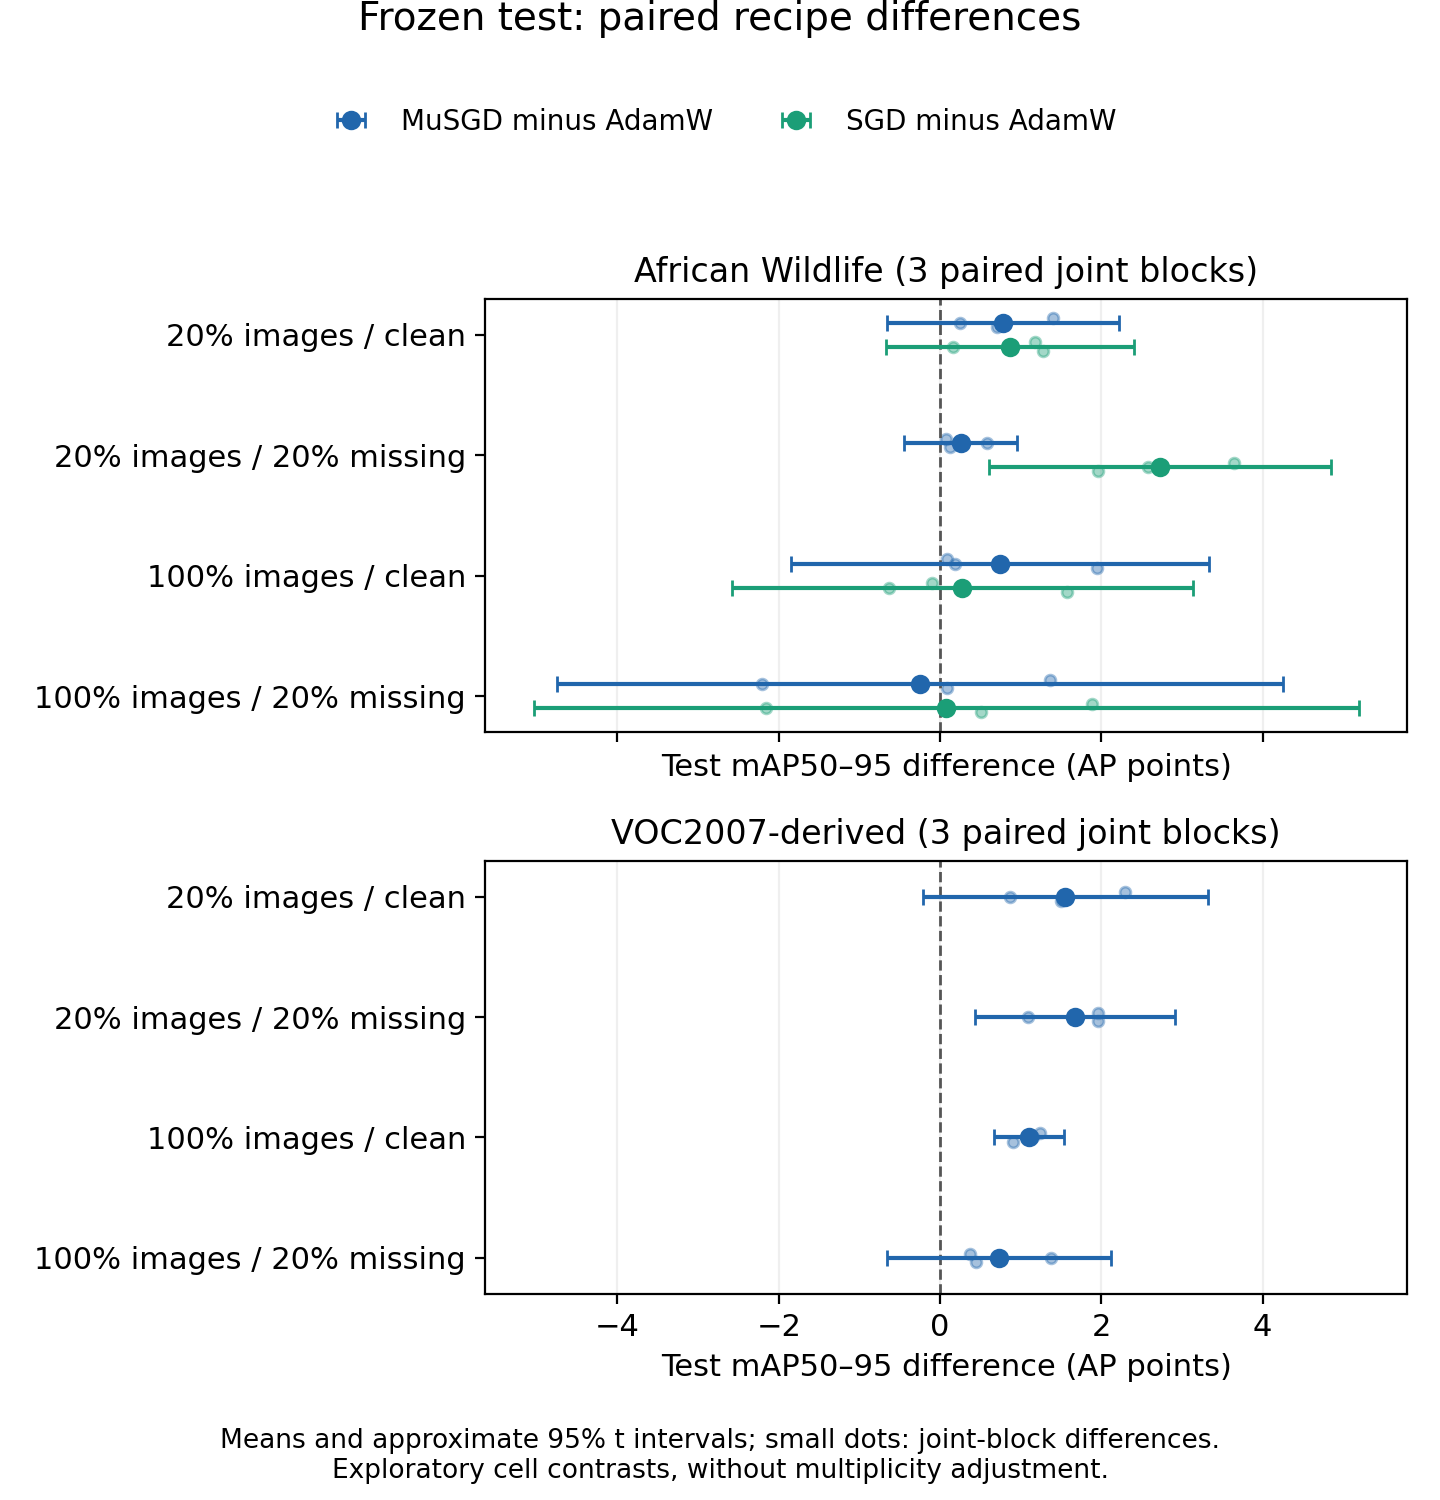
\includegraphics[width=\linewidth]{images/journal_test_contrasts.png}
\caption{Paired frozen-test recipe differences across three joint blocks. Large points denote means, error bars are approximate unadjusted 95\% Student $t$ intervals, and small points show block values. Positive values favor the named recipe over AdamW. SGD is included only on wildlife. The figure reports cell contrasts, not the three-way interaction.}
\end{figure}
On wildlife, MuSGD--AdamW mean test differences are $+0.79$, $+0.26$, $+0.74$ and $-0.25$ AP points for scarce/clean, scarce/missing, full/clean and full/missing conditions. All four approximate paired intervals include zero. On VOC-derived data the corresponding differences are $+1.55$, $+1.67$, $+1.10$ and $+0.73$ points. The intervals for scarce/missing and full/clean exclude zero before any multiplicity correction; these remain exploratory cell comparisons across only three joint blocks.

The prespecified MuSGD--AdamW three-way contrast is $+0.470$ points on wildlife, with interval $[-6.383,7.322]$, and $+0.488$ on VOC-derived data, with interval $[-0.660,1.637]$. Both intervals include zero. The small joint-block sample leaves the scarcity--missingness interaction unresolved. SGD is a substantive secondary comparator: its wildlife scarce/missing test point estimate exceeds AdamW by $+2.73$ points (unadjusted interval $[0.61,4.85]$), while the remaining SGD--AdamW cell intervals include zero. SGD therefore remains a competitive comparator in the evaluated setting.

\subsection{One-block sensitivity checks}
For block 101 with missing boxes, moving from 20 to 60 exposure blocks lowered best-checkpoint clean-validation mAP in all four transferred-settings comparisons: by 2.11/3.51 points for AdamW at scarce/full data, and 0.65/2.06 for MuSGD. Best epochs in the longer runs ranged from 36 to 51. The horizon and schedules changed together, and settings were selected at ten blocks; these results do not identify a converged optimum.

Replacing MuSGD's native $3\times$ head LR with $1\times$, at the same selected base LR and block 101, changed clean-validation AP by $+1.56$, $+1.41$, $+0.08$ and $-0.04$ across the four conditions. These are one-block validation checks without additional test scoring or independent retuning. Their sensitivity reinforces the need to interpret native recipe differences rather than assigning effects to orthogonalization alone.

\section{Discussion and limitations}
The measured effects are dataset- and split-dependent. Wildlife validation favored AdamW over MuSGD in both scarce-data conditions, whereas wildlife test point estimates slightly favored MuSGD there; the test intervals include zero. VOC-derived test point estimates favored MuSGD in all four conditions, but the three-way contrast remained uncertain. The original pilot's scarcity-specific advantage therefore does not support a general interaction claim across these controlled comparisons.

Exposure matching holds presented images and updates constant across unique-image fractions, but it does not remove search-boundary limitations, native recipe differences or held-out sample variation. In particular, all selected rates are lower-bound optima within the searched grids. A stronger claim about optimized-recipe rankings requires wider validation search under a new prospective evaluation design; the current opened test split must not guide a new confirmatory search.

Limits include lower-bound learning-rate selection without the planned extension, the shorter tuning horizon, one tuning randomization, three confirmation blocks, synthetic independent deletion, retained annotation errors, residual scene overlap, possible pretrained-image overlap and native optimizer implementation differences. The joint-block intervals capture neither image-sampling uncertainty in fixed held-out splits nor separate variance components of subset, deletion and training seeds. Equal candidate counts do not guarantee equal tuning-time or search-coverage fairness. The VOC-derived all-object task is explicitly distinct from standard VOC scoring. A single small detector and two datasets limit generalization. Source photographs are not included in the manuscript or companion source bundle.

\section{Code and data availability}
The public Kaggle notebook is available at
\url{https://www.kaggle.com/code/myudak/muon-yolo-journal}.
The completed experimental run and its outputs are preserved in version~1:
\url{https://www.kaggle.com/code/myudak/muon-yolo-journal?scriptVersionId=361947826}.
Later visibility or presentation saves do not replace that evidence.

The notebook embeds source, tests and frozen configuration with integrity checks. Its outputs include source and variant fingerprints, checkpoint lineage, an environment lock, optimizer groups, actual update counts, image-order hashes, histories, metric records and the final checkpoint freeze. Principal evidence files are \texttt{results.json}, \texttt{campaign\_summary.json}, \texttt{frozen\_final\_test\_plan.json}, and \texttt{final\_test\_results.json}, under \texttt{muon\_yolo\_journal/}. The compact evidence audit verifies recorded identities and internal consistency; independent rehashing of source-image and checkpoint bytes requires those larger artifacts.

African Wildlife and VOC images remain third-party data subject to their source terms \cite{wildlifeData,everingham2010}. The paper contains numerical figures rather than source photographs. Upstream software and model licenses retain their own terms.

\section{Conclusion}
Under the evaluated fixed-update fine-tuning budget, MuSGD produced modest positive test point differences on VOC-derived data and smaller, mixed differences on wildlife. The primary scarcity--missingness interaction remained uncertain on both datasets. Completed SGD and head-LR checks further constrain a simple MuSGD-superiority interpretation. The reproducible outcome is a conditional recipe comparison with explicit exposure and search boundaries; stronger generalization requires wider validation search and more independent evidence.

\appendix
\section{Development pilot}
\begin{table}[ht]
\centering
\caption{Measured pilot validation mAP50--95 multiplied by 100. One joint block, untuned rates, fixed ordinary epochs. $\Delta$ is MuSGD minus AdamW in AP points. These are not journal confirmation or test results.}
\begin{tabular}{rrrrr}
\toprule
Images & Target missing boxes & AdamW & MuSGD & $\Delta$\\
\midrule
205 & 0\% & 69.83 & 70.60 & $+0.76$\\
205 & 20\% & 65.91 & 68.23 & $+2.32$\\
1,021 & 0\% & 79.68 & 77.26 & $-2.42$\\
1,021 & 20\% & 74.80 & 72.53 & $-2.27$\\
\bottomrule
\end{tabular}
\end{table}

The optimizer ranking reverses across fractions under these provisional settings. The single-block three-way contrast is $+1.413$ AP points, with no estimated confidence interval. Realized deletion was 72/385 boxes (18.70\%) in the scarce subset and 361/1,881 (19.19\%) in the full pool.

At 20 ordinary epochs, scarce runs saw 4,100 images and 260 updates, while full-data runs saw 20,420 images and 1,280 updates. Seven of eight runs attained their best per-epoch validation mAP at epoch 20; the remaining run did so at epoch 19. The observations therefore neither establish convergence nor separate unique-image scarcity from update exposure. They motivate the later controlled campaign rather than confirm its hypothesis. No test metric was computed in the pilot.


\section{Complete paired estimates}
\begingroup\small
All estimates below use joint blocks 101--103. Differences and approximate unadjusted 95\% Student $t$ intervals are in AP points. The three-way contrast follows the definition in the main text.
\Needspace{20\baselineskip}
\subsection{African Wildlife: validation}
\begin{longtable}{@{}lrrrr@{}}
\caption{African Wildlife: validation paired recipe differences.}\\
\toprule Recipe versus AdamW & Images & Missing & Mean & 95\% interval\\\midrule
\endfirsthead
\toprule Recipe versus AdamW & Images & Missing & Mean & 95\% interval\\\midrule
\endhead
MuSGD & 20\% & 0\% & -0.71 & [-4.22, 2.80]\\
SGD & 20\% & 0\% & +0.72 & [-2.96, 4.40]\\
MuSGD & 20\% & 20\% & -1.37 & [-3.32, 0.59]\\
SGD & 20\% & 20\% & +0.01 & [-2.04, 2.05]\\
MuSGD & 100\% & 0\% & -0.17 & [-1.12, 0.77]\\
SGD & 100\% & 0\% & +0.66 & [-1.36, 2.69]\\
MuSGD & 100\% & 20\% & +0.62 & [0.07, 1.17]\\
SGD & 100\% & 20\% & +0.99 & [-0.72, 2.70]\\
\bottomrule\end{longtable}
MuSGD--AdamW three-way contrast: $-1.451$ AP points; approximate 95\% interval $[-5.864, 2.963]$.
SGD--AdamW three-way contrast: $-1.038$ AP points; approximate 95\% interval $[-6.673, 4.596]$.
\Needspace{14\baselineskip}
\subsection{VOC2007-derived: validation}
\begin{longtable}{@{}lrrrr@{}}
\caption{VOC2007-derived: validation paired recipe differences.}\\
\toprule Recipe versus AdamW & Images & Missing & Mean & 95\% interval\\\midrule
\endfirsthead
\toprule Recipe versus AdamW & Images & Missing & Mean & 95\% interval\\\midrule
\endhead
MuSGD & 20\% & 0\% & +1.79 & [-0.04, 3.62]\\
MuSGD & 20\% & 20\% & +1.48 & [0.31, 2.65]\\
MuSGD & 100\% & 0\% & +0.74 & [-0.89, 2.38]\\
MuSGD & 100\% & 20\% & +1.64 & [-0.99, 4.26]\\
\bottomrule\end{longtable}
MuSGD--AdamW three-way contrast: $-1.199$ AP points; approximate 95\% interval $[-6.280, 3.883]$.
\Needspace{20\baselineskip}
\subsection{African Wildlife: frozen test}
\begin{longtable}{@{}lrrrr@{}}
\caption{African Wildlife: frozen test paired recipe differences.}\\
\toprule Recipe versus AdamW & Images & Missing & Mean & 95\% interval\\\midrule
\endfirsthead
\toprule Recipe versus AdamW & Images & Missing & Mean & 95\% interval\\\midrule
\endhead
MuSGD & 20\% & 0\% & +0.79 & [-0.66, 2.23]\\
SGD & 20\% & 0\% & +0.87 & [-0.67, 2.41]\\
MuSGD & 20\% & 20\% & +0.26 & [-0.44, 0.96]\\
SGD & 20\% & 20\% & +2.73 & [0.61, 4.85]\\
MuSGD & 100\% & 0\% & +0.74 & [-1.85, 3.34]\\
SGD & 100\% & 0\% & +0.28 & [-2.58, 3.14]\\
MuSGD & 100\% & 20\% & -0.25 & [-4.75, 4.25]\\
SGD & 100\% & 20\% & +0.08 & [-5.04, 5.19]\\
\bottomrule\end{longtable}
MuSGD--AdamW three-way contrast: $+0.470$ AP points; approximate 95\% interval $[-6.383, 7.322]$.
SGD--AdamW three-way contrast: $+2.059$ AP points; approximate 95\% interval $[-2.292, 6.410]$.
\Needspace{14\baselineskip}
\subsection{VOC2007-derived: frozen test}
\begin{longtable}{@{}lrrrr@{}}
\caption{VOC2007-derived: frozen test paired recipe differences.}\\
\toprule Recipe versus AdamW & Images & Missing & Mean & 95\% interval\\\midrule
\endfirsthead
\toprule Recipe versus AdamW & Images & Missing & Mean & 95\% interval\\\midrule
\endhead
MuSGD & 20\% & 0\% & +1.55 & [-0.21, 3.32]\\
MuSGD & 20\% & 20\% & +1.67 & [0.43, 2.91]\\
MuSGD & 100\% & 0\% & +1.10 & [0.67, 1.54]\\
MuSGD & 100\% & 20\% & +0.73 & [-0.66, 2.12]\\
\bottomrule\end{longtable}
MuSGD--AdamW three-way contrast: $+0.488$ AP points; approximate 95\% interval $[-0.660, 1.637]$.

\endgroup

\begin{thebibliography}{99}
\bibitem{yang2020} Y. Yang, K. J. Liang and L. Carin. \emph{Object Detection as a Positive-Unlabeled Problem}. BMVC, 2020. \url{https://arxiv.org/abs/2002.04672}.
\bibitem{jordan2024} K. Jordan. \emph{Muon: An optimizer for hidden layers in neural networks}. 2024. \url{https://kellerjordan.github.io/posts/muon/}.
\bibitem{jocher2026} G. Jocher et al. \emph{Ultralytics YOLO26: Unified Real-Time End-to-End Vision Models}. arXiv:2606.03748, 2026. \url{https://arxiv.org/abs/2606.03748}.
\bibitem{huang2026} F. Huang, Y. Luo and S. Chen. \emph{MiMuon: Mixed Muon Optimizer with Improved Generalization for Large Models}. arXiv:2605.19619, 2026. \url{https://arxiv.org/abs/2605.19619}.
\bibitem{akhtar2026} M. Akhtar et al. \emph{When Does Muon Actually Win? A Paired Data-, Time-, and Tuning-Budget Benchmark}. arXiv:2610.21555, 2026. \url{https://arxiv.org/abs/2610.21555}.
\bibitem{ruan2026} T. Ruan, F. Zhang, S. Wang and S. Zhang. \emph{Muon Learns More Robust and Transferable Features than Adam}. arXiv:2606.09658, 2026. \url{https://arxiv.org/abs/2606.09658}.
\bibitem{qu2026} X. Qu, H. Peigeng and S. Horv\'ath. \emph{Can Muon Fine-tune Adam-Pretrained Models?} Proceedings of the 43rd International Conference on Machine Learning, PMLR 306:102619--102650, 2026. \url{https://proceedings.mlr.press/v306/qu26e.html}.
\bibitem{penquitt2026} S. Penquitt et al. \emph{Object Detection Benchmarks are Incomplete: The Role of Label Errors and Annotation Uncertainty}. arXiv:2609.21822, 2026. \url{https://arxiv.org/abs/2609.21822}.
\bibitem{everingham2010} M. Everingham, L. Van Gool, C. K. I. Williams, J. Winn and A. Zisserman. \emph{The Pascal Visual Object Classes (VOC) Challenge}. International Journal of Computer Vision, 88:303--338, 2010. \url{https://doi.org/10.1007/s11263-009-0275-4}.
\bibitem{wildlifeData} Ultralytics. \emph{African Wildlife Detection Dataset}. Dataset documentation, accessed 31 October 2026. \url{https://docs.ultralytics.com/datasets/detect/african-wildlife/}.
\end{thebibliography}
\end{document}
